\documentclass[a4paper,12pt]{article}

\usepackage[utf8]{inputenc}
\usepackage[T1]{fontenc}
\usepackage[frenchb]{babel}
\usepackage{a4wide}
\usepackage{graphicx}
\usepackage{subfig}
\usepackage{tikz}
\usepackage{ifthen}
\usepackage{ifpdf}
\usepackage{comment}
\usepackage{listings} % pour code XML


\graphicspath{{images/}}

\newlength\figureheight
\newlength\figurewidth

\ifpdf
\usepackage[pdftex]{hyperref}
\else
\usepackage{hyperref}
\fi

\usepackage{color}
\hypersetup{
colorlinks=true,
linkcolor=black,
citecolor=black,
urlcolor=black}

\renewcommand{\baselinestretch}{1.05}
\usepackage{fancyhdr}
\pagestyle{fancy}
\fancyfoot{}
\fancyhead[LE,RO]{\bfseries\thepage}
\fancyhead[RE]{\bfseries\nouppercase{\leftmark}}
\fancyhead[LO]{\bfseries\nouppercase{\rightmark}}
\setlength{\headheight}{15pt}

\let\headruleORIG\headrule
\renewcommand{\headrule}{\color{black} \headruleORIG}
\renewcommand{\headrulewidth}{1.0pt}
\usepackage{colortbl}
\arrayrulecolor{black}

\fancypagestyle{plain}{
  \fancyhead{}
  \fancyfoot[C]{\thepage}
  \renewcommand{\headrulewidth}{0pt}
}

\makeatletter
\def\cleardoublepage{\clearpage\if@twoside \ifodd\c@page\else
  \hbox{}
  \thispagestyle{empty}
  \newpage
  \if@twocolumn\hbox{}\newpage\fi\fi\fi}
\makeatother

\parskip=5pt

\usepackage{amsthm}
\usepackage{array}
\usepackage{bm}

\lstset{ % encadrer et coloriser un document XML
  language=xml,frame=single, 
  breaklines=true, 
  basicstyle=\ttfamily,
  basicstyle=\scriptsize, 
  keywordstyle=\color{blue}, 
  commentstyle=\color{green}, 
  stringstyle=\color{red}, 
  identifierstyle=\color{blue}
}


\begin{document}

%%%%%%%%%%%%%%%%%%%%%%%%%%%%%%%%%%%%%%%%%%%%  page de garde  %%%%%%%%%%%%%%%%%%

\begin{titlepage}
\begin{center}

\begin{minipage}[c]{.46\linewidth}
  \centering
  
\includegraphics[width=0.6\textwidth]{logo_UPMC.png}\\[1cm]
\end{minipage}
\hfill
\begin{minipage}[c]{.46\linewidth}
  \centering
  
\includegraphics[width=0.3\textwidth]{logo_lip6.png}\\[1cm]
\end{minipage}

\vspace*{1cm}

{\large Université Pierre et Marie Curie}\\[1cm]

{\large Master Informatique, Spécialité STL}\\[1cm]

{\large Semestre 2, UE Projet STL}\\[1cm]

% titre
\rule{\linewidth}{0.5mm} \\[0.5cm]
{ \huge \bfseries Un analyseur syntaxique pour MusicXML \\[0.4cm] }
\rule{\linewidth}{0.5mm} \\[0.5cm]

\vspace*{1cm}

% Auteurs
\noindent
\begin{minipage}{0.5\textwidth}
  \begin{flushleft} \large
    \emph{Auteurs :}\\
      Sébastien \textsc{Duchenne}\\
      Alexandre \textsc{Gaspard Cilia}\\~\\
    \emph{Encadrant :} \\
    Pr.~Carlos \textsc{Agon}\\
  \end{flushleft}
\end{minipage}

\vspace*{2cm}

{\large Soutenue le xx xx 2017}\\[1cm]

\vfill

\end{center}
\end{titlepage}

\tableofcontents

\newpage

%%%%%%%%%%%%%%%%%%%%%%%%%%%%%%%%%%%%%%%%%%%%%%%  Remerciements  %%%%%%%%%%%%%%%%%%%%


%\begin{acknowledgements}
%\addchaptertocentry{\acknowledgementname} % Add the acknowledgements to the table of contents
%The acknowledgments and the people to thank go here, don't forget to include your project advisor\ldots
%\end{acknowledgements}


%%%%%%%%%%%%%%%%%%%%%%%%%%%%%%%%%%%%%%%%%%%%%%%  Liste des figures  %%%%%%%%%%%%%%%%%%%%


\listoffigures % liste des figures


%%%%%%%%%%%%%%%%%%%%%%%%%%%%%%%%%%%%%%%%%%%%%%%  Abbréviation  %%%%%%%%%%%%%%%%%%%%

%\begin{abbreviations}{ll} % liste des abbréviations

%\textbf{DOM} & \textbf{Document} \textbf{O}bject \textbf{M}odel\\
%\textbf{XML} & E\textbf{x}tensible \textbf{M}arkup \textbf{L}angage\\

%\end{abbreviations}


%%%%%%%%%%%%%%%%%%%%%%%%%%%%%%%%%%%%%%%%%%%%%%%  Contenu  %%%%%%%%%%%%%%%%%%%%


\pagestyle{fancy}

\section{Introduction}


L'IRCAM \cite{ircam}, Institut de Recherche et Coordination en Acoustique/Musique, est un centre de création et de recherche scientifique sur la musique. Il a été fondé en 1969 par Pierre Boulez à la demande du président Georges Pompidou. 

\par
En 1995, le CNRS et le ministère de la Culture et de la Communication s'associe et créée l'UMR 9912 STMS. Cette unité mixte de recherche, hébergée à l'IRCAM, s'intéressent aux sciences et aux technologies de la musique et du son. En 2010, elle est rejoint par l'UPMC.

\par
Cette UMR est composé de nombreuses équipes de recherche. L'une d'elles s'intitule "Représentation musicale", et réalise des outils de compositions musicales. Elle a notamment créée OpenMusic \cite{openmusic}, un environnement de composition musicale assisté par ordinateur.

\par
Les chercheurs de l'IRCAM souhaitent travailler sur des partitions musicales sous formes d'arbres rythmiques. Actuellement, ils utilisent OpenMusic. Cependant, ce logiciel --- (mettre inconvénients) ---. C'est pourquoi, ils souhaitent une nouvelle version. 

\par
Ce programme sera écrit en langage Java et sera similaire à OpenMusic. Il permettra donc d'éditer graphiquement des morceaux de musique. Son implémentation comportera différents modules, dont celui consistant à construire les arbres rythmiques à partir d'un fichier au format MusicXML. C'est ce module que notre tuteur de projet Carlos Agon, enseignant-chercheur à l'UPMC et membre de l'équipe de représentation musicale, nous a demandé de réaliser.

\par
Le module que nous avons développé est déposé sur un compte GitHub \cite{github_pstl}.

\section{Technologies utilisées}

\subsection{OpenMusic}

OpenMusic \cite{openmusic} est un langage de programmation visuel basé sur le langage Lisp qui permet d'écrire graphiquement des compositions musicales. Il a été conçu par les chercheurs de l'IRCAM Carlos Agon, Gérard Assayag et Jean Bresson. Les programmes sont constitués d'éléments reliés entre eux et représentant des structures de données ou des fonctions. La figure suivante montre l'interface du logiciel.


\begin{figure}[!h] %h : here
\centering
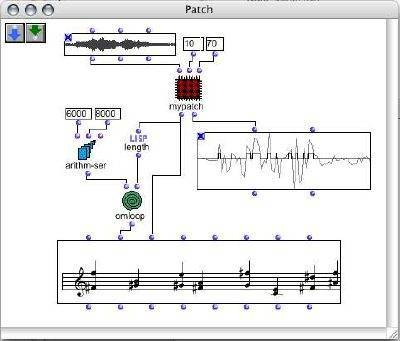
\includegraphics[width=0.8\textwidth]{openmusic.jpg}\\[1cm]
\caption{OpenMusic}
\label{OpenMusic}
\end{figure}

\par
Dans ce logiciel, les morceaux de musique sont constitués d'une suite d'arbres rythmiques. Comme décrit dans l'article \cite{agon}, \enquote{un arbre rythmique est défini comme un couple (D S) où D est une fraction (< 0) et S est une liste de n-éléments définissant n-proportions de D. Chaque élément de S peut-être soit un entier, soit un arbre rythmique.}

\par
Les images suivantes sont des exemples d'arbres rythmiques, en haut, et la partition correspondante, en bas.


\begin{minipage}[c]{.46\linewidth}
  \centering
  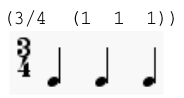
\includegraphics[width=0.5\textwidth]{rt1.png}\\[1cm]
\end{minipage}
\hfill
\begin{minipage}[c]{.46\linewidth}
  \centering
  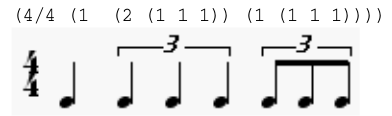
\includegraphics[width=0.9\textwidth]{rt2.png}\\[1cm]
\end{minipage}



\subsection{Le langage Java}

\par 
Java est un langage de programmation \textbf{orienté objet} fortement typé développé par \textbf{Sun Microsystems} à partir de \textbf{1995}. La société sera plus tard rachetée par \textbf{Oracle} en 2009 qui possède et maintient Java encore aujourd'hui.

\par 
Java se détache de la masse des autres langages de programmation notamment grâce à sa portabilité et sa facilité d'utilisation.

\begin{lstlisting}[caption=Hello world en java]
public class HelloWorld {
    public static void main(String[] args) {
        System.out.println("Hello world!");
    }
}
\end{lstlisting}

\par
Ci-dessus, un classique "Hello world" en Java. Nous pouvons y voir la définition de la classe \emph{HelloWorld} ainsi que la méthode principale du programme nommé \emph{main} et enfin un affichage sur la sortie standard.



\subsection{Le format MusicXML}

MusicXML \cite{musicxml} est un format de fichier permettant de représenter la notation musicale occidentale (notation classique, accords en notation anglo-saxonne, tablatures et percussions) et basé sur le langage XML. Il est propriétaire mais il peut librement utilisé avec une licence publique.

\par
Il y a plus de 20 ans, le format MIDI était très utilisé. Cependant, il n’est pas très adapté pour représenter toutes les caractéristiques de la musique, on perd donc en informations avec ce format. Pour pallier à cela, les formats SMDL et NIFF ont été créés. Cependant, le format SMDL était complexe et donc peu compréhensible. Il était donc très peu utilisé. Le format NIFF était un format peu pratique à utiliser et n’a donc pas été adopté par certains logiciels. Ces formats n’ont donc pas eu le succès souhaité.

\par
En 2004, la société Recordare LLC s’inspire des 2 formats universitaires MuseData et Humdrum pour créer la première version du format MusicXML. Ses avantages sont qu’il est facile à manipuler. Il permet le transfert de morceaux de musique d’une application à une autre. Il peut représenter beaucoup de caractéristiques de la musique. Cependant, il est verbeux, puisqu'il utilise le format XML, et ne donc permet pas de représenter la musique non occidentale.

\par
Il est de plus en plus utilisé puisque plus de 200 logiciels de musique l’ont adopté. Il est donc possible de travailler finement sur un morceau de musique en utilisant différents programmes.

\par
Comme le format XML est verbeux, le fichier prend de la place. La version 2.0, sortie en 2007, apporte donc la compression du fichier au format xml en un fichier au format mxl, et permet de diviser sa taille de façon importante. La version 3.0, sortie en 2011, permet le support des instruments virtuels.\\~\\

\par
On voit, dans le code correspondant à la partition suivante, que les informations sur la partition sont placées dans la balise "measure" et celle concernant la ronde sont contenues dans la balise "note".

\begin{figure}[!h] %h : here
\centering
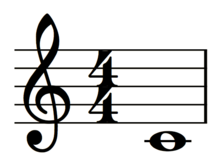
\includegraphics[width=0.2\textwidth]{musicxml_hello_world.png}\\[1cm]
%source : https://en.wikipedia.org/wiki/MusicXML
\caption{Hello World en MusicXML}
\label{Hello World en MusicXML}
\end{figure}


\begin{lstlisting}[caption=Document XML d'un Hello World en MusicXML, label=ruleml]
<?xml version="1.0" encoding="UTF-8" standalone="no"?>
<!DOCTYPE score-partwise PUBLIC
    "-//Recordare//DTD MusicXML 3.0 Partwise//EN"
    "http://www.musicxml.org/dtds/partwise.dtd">
<score-partwise version="3.0">
  <part-list>
    <score-part id="P1">
      <part-name>Music</part-name>
    </score-part>
  </part-list>
  <part id="P1">
    <measure number="1">
      <attributes>
        <divisions>1</divisions>
        <key>
          <fifths>0</fifths>
        </key>
        <time>
          <beats>4</beats>
          <beat-type>4</beat-type>
        </time>
        <clef>
          <sign>G</sign>
          <line>2</line>
        </clef>
      </attributes>
      <note>
        <pitch>
          <step>C</step>
          <octave>4</octave>
        </pitch>
        <duration>4</duration>
        <type>whole</type>
      </note>
    </measure>
  </part>
</score-partwise>
\end{lstlisting}



\subsection{Le langage XML}

Le langage XML \cite{xml_w3c, xml_ocr}, acronyme de e\textbf{X}tensible \textbf{M}arkup \textbf{L}angage, est langage de balisage générique spécifié par le W3C. Il permet de définir différents espaces de noms, c'est à dire des langages avec leur propre grammaire et vocabulaire. Il permet l'échange d'information entre des programmes très différents à condition d'utiliser la même grammaire.

\par
Il a l'avantage de pouvoir être compris par les êtres humains et les machines. Cependant, c'est un langage verbeux et qui peut donc prendre beaucoup de place s'il contient beaucoup d'information.

\par
Un document XML est constitué de balises pouvant contenir d'autres balises ou une valeur simple. Une balise peut aussi contenir des attributs donnant des informations supplémentaires sur le contenu.

\begin{lstlisting}[caption=Exemple d'un document XML]
<?xml version="1.0" encoding="UTF-8"?>
<racine>
    <balise attribut="valeur" >Contenu</balise>
    <baliseunique />
</racine>
\end{lstlisting}

\par
Ci-dessus un exemple de XML simpliste mais qui met en avant les bases du langage. La première ligne annonce le type de document et la version dans lequel le document va être rédigé. \emph{<racine>} est le nœud racine du document, celui qui en somme va contenir tout le document. On peut ici, facilement remarquer que le document peut être représenté sous la forme d'un arbre.

\par
XML permet à l'utilisateur de définir lui même la grammaire de son document grâce notamment aux \textbf{DTD} et au \textbf{Schéma XML}. Ces outils nous permettent de disposer de format d’échange de données tel que \textbf{MusicXML}.


\subsection{Le langage Relax NG}

\textbf{Relax NG} (\textbf{Re}gular \textbf{La}nguage for \textbf{X}ML \textbf{N}ext \textbf{G}eneration) née de la fusion de TreX de James Clark et de Relax de Murata Makoto. C'est un langage qui permet de définir la grammaire d'un document XML. Relax NG ne s'intéresse qu'à la structure du document et non à sa valeur.

\par
C'est ce que nous utiliserons afin de s'assurer de la validité du document à traiter.


\subsection{Affichage d'un graphe avec GraphStream}

Une fois le fichier XML parsé, nous disposons d'un \emph{DOM} sous forme d'un objet \emph{document}. Nous pouvons ensuite afficher l'arbre grâce à la librairie GraphStream \cite{graphstream}. Pour cela nous appelons un méthode qui affiche un nœud de l'arbre sur la racine du \emph{Document}. Cela nous permet donc d'afficher tout l'arbre.


\subsection{Les librairies}

Dans cette section, nous aborderons les librairies utilisées pour réaliser ce projet. Cela ira de la validation du XML en passant par le parsing de ce dernier, jusqu'à la récupération des information stockées dans le fichier MusicXML.


\subsubsection{Trang et Jing}

\textbf{Trang} \cite{trang} et \textbf{Jing} \cite{jing} sont deux librairies développées par \textbf{Thai Open Source}. Elles permettant de générer des grammaires Relax NG et de valider des documents XML à partir de cette même grammaire.

\par
Trang est une librairie qui permet de traduire un fichier de description grammaticale en fichier Relax NG. En effet XML n'est pas facilement lisible pour un esprit humain, c'est pour cela que Trang nous permet de créer notre grammaire dans un langage plus compréhensible. Une fois la grammaire écrite dans un fichier en \emph{.rnc}, nous pouvons générer notre fichier Relax NG en \emph{.rng}.

\par
Jing, quant à lui, est une librairie Java qui permet de valider un document XML à l'aide d'un fichier Relax NG.


\begin{lstlisting}[caption=Code java permettant de vérifier la validation d'un document XML]

final ValidationDriver vd = new ValidationDriver();
vd.loadSchema(rngFile);

if (!vd.validate(inputTextStream)) {
	throw new ParseException("Invalid xml :(");
} else {
    System.out.println("Valid xml :)");
}
\end{lstlisting}

\par
Le code ci-dessus est une utilisation simplifiée de Jing. Nous commençons tout d'abord par créer un objet \emph{ValidationDriver} de Jing dans lequel nous chargeons notre fichier Relax NG. Nous n'avons ensuite plus qu'à lancer la méthode \emph{validate(InputSource in) : boolean} qui nous indiquera si le document est valide.


\subsubsection{L'API SAX}

SAX \cite{sax_website, sax_oracle} est une API créée par David Megginson en 1998 et est l'acronyme de \textbf{S}imple \textbf{A}PI for \textbf{X}ML. Elle permet de manipuler des documents XML en utilisant des événements envoyées à chaque rencontre d'un élément.


\subsubsection{Le DOM}

Le DOM \cite{dom_w3c} , ou \textbf{D}ocument \textbf{O}bject \textbf{M}odel, est une interface de programmation normalisée par le W3C et est indépendant de tout plateforme et langage. Il voit les documents à balises comme des arbres dont le contenu et la structure peuvent être accédés et mis à jour dynamiquement.

\par
La figure suivante montre un exemple de DOM.

\begin{figure}[!h]
\centering
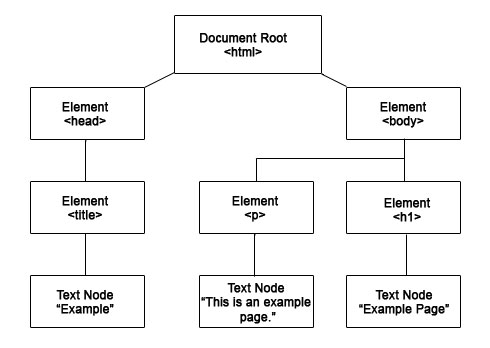
\includegraphics[width=0.8\textwidth]{ex_dom.jpg}\\[1cm]
%source : http://www.computerhope.com/jargon/d/dom.htm
\caption{Exemple d'un DOM}
\label{Exemple d'un DOM}
\end{figure}


\section{Autre section}

\subsection{Parsing d'un fichier MusicXML}

Un document XML est chargé puis vérifié grâce à la grammaire de MusicXML. Si le document est conforme, il est parsé en DOM ce qui permet de travailler dessus facilement.

\begin{figure}[!h]
\centering
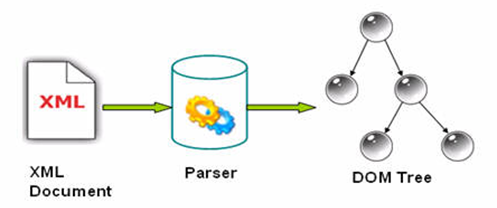
\includegraphics[width=0.5\textwidth]{parsing_xml_to_dom.png}\\[1cm]
%source : http://www.amfastech.com/2014/11/complete-tutorial-on-selecting-best-xml-parser.html
\caption{Parsing d'un document XML en DOM}
\label{Parsing d'un document XML en DOM}
\end{figure}



\subsection{Composition d'un morceau}


Un morceau est composé de plusieurs portées et/ou plusieurs systèmes de portée.
\par
Un système de portée est constitué de portées.
\par
Une porté est liée à un instrument et est composée d’une clé, d’une armure, d’un chiffrage de la mesure et de mesure.
\par
Une clé contient un nom et un numéro de ligne.
\par
Une armure est composée d'un nombre entier relatif. S'il est négatif alors l'armure contient des bémols, s'il est positif alors elle contient des dièses, s'il vaut 0 alors rien n'est affiché.
\par
Le chiffrage de la mesure contient un numérateur, représentant le nombre de temps de la mesure, et dénominateur, représentant la durée d’une mesure.
\par
Une mesure est composée d'une clé optionnelle, d'un chiffrage de la mesure optionnel, de notes, de notes reliées par une division artificielle du temps (duolet/triolet/quartolet/...), d'accords, de silences, de notes reliées par une liaison, de signes indiquant si la mesure est répétée et comment et de notes jouées en crescendo / decrescendo.
\par
Une note est constituée d'un nom, d'une série, d'une durée, d'une proportion par rapport à la ronde, d'un point indiquant si elle est pointée ou pas, d'un volume, de paroles et d'une altération (bémol, dièse ou remise à la normal).
\par
Un silence est composé d'un nom, d'une série, d'une durée, d'une proportion par rapport à la ronde et d'un point indiquant si elle est pointée ou pas.

%Récapitulatif sous forme de liste:\\
%\begin{itemize}
%\item morceau : plusieurs portées et/ou plusieurs systèmes de portée
%\item système de portée : portées
%\item une porté est lié à un instrument et est composée d’une clé, d’une armure, d’un chiffrage de la mesure et de mesure
%\item clé : nom et numéro de ligne
%\item armure : nombre entier relatif, négatif : bémol, positif : dièse
%\item chiffrage de la mesure : numérateur représentant le nombre de temps de la mesure et dénominateur représentant la durée d’une mesure
%\item mesure : clé optionnelle, chiffrage de la mesure optionnel, notes, notes reliées par une division artificielle du temps (duolet/triolet/quartolet/...), accords, silences, notes reliées par une liaison, si la mesure est répétée et comment, notes jouées en crescendo / decrescendo
%\item note : nom, série, durée, proportion par rapport à la ronde, pointée ou pas, volume, paroles, altération (bémol, dièse ou normal), tiret
%\item silence : nom, série, durée, proportion par rapport à la ronde, pointée ou pas
%\end{itemize}
%\section{Conclusion}

conclusion


%%%%%%%%%%%%%%%%%%%%%%%%%%%%%%%%%%%%%%%%%%%%%%%  Annexes  %%%%%%%%%%%%%%%%%%%%

%\appendix %

%\include{annexes}


%%%%%%%%%%%%%%%%%%%%%%%%%%%%%%%%%%%%%%%%%%%%%%%  Bibliographie  %%%%%%%%%%%%%%%%%%%%

\bibliographystyle{authoryear-fr}
\bibliography{biblio}
\nocite{*}

\end{document}